\documentclass[aps,prl,twocolumn,superscriptaddress]{revtex4}

\usepackage[strict]{revquantum}   


%% PATHS %%

\newcommand{\figurefolder}{../fig}


%% OTHER NOTATION %%

% Normalize spelling, font decoration.
\newcommand{\mps}{x}
\newcommand{\eps}{e}
\newcommand{\data}{d}

\newcommand{\MLE}{\text{MLE}}


% http://tex.stackexchange.com/a/112947/615
\newcommand{\apxref}[1]{\hyperref[#1]{Appendix~\ref{#1}}}

%=============================================================================
% FRONT MATTER
%=============================================================================

\begin{document}

\title{Adaptive Online Experiment Design with Quantum Systems}

\author{Ian Hincks}
\affilUWAMath
\affilIQC

\author{Thomas Alexander}
\affilUWPhys
\affilIQC

\author{Michal Kononenko}
\affilTODO

\author{Benjamin Soloway}
\affilTODO

\author{David G. Cory}
\affilUWChem
\affilIQC
\affilPI

% new authors add your names

\date{\today}

\begin{abstract}
    Aliquam maximus sem ut imperdiet pulvinar. Donec ut sagittis metus, vitae congue risus. Vestibulum ut mi pharetra, commodo risus eget, consequat sapien. Integer vulputate dolor nec nisl sodales, quis condimentum nulla mollis. Curabitur molestie lacus eget accumsan elementum. 
\end{abstract}

\maketitle

%=============================================================================
% MAIN DOCUMENT
%=============================================================================



%=============================================================================
\section{Introduction}
\label{sec:intro}
%=============================================================================

 Lorem ipsum dolor sit amet, consectetur adipiscing elit. Pellentesque quis tellus in lorem fermentum vehicula. Cras placerat ante arcu, vitae porta felis sodales ac. Orci varius natoque penatibus et magnis dis parturient montes, nascetur ridiculus mus. Fusce turpis velit, mattis vel lectus nec, aliquam molestie ligula. Nam sollicitudin, urna cursus ultricies molestie, orci metus aliquet odio, vel consectetur augue tortor in neque. Donec posuere diam nec ligula laoreet fringilla. Proin diam dui, hendrerit eu tortor vel, ultrices maximus mi. Phasellus sodales finibus massa nec porttitor. Ut posuere tortor id ante lobortis iaculis at at ex. Phasellus in ligula suscipit, pulvinar est at, mollis est. Fusce rutrum pretium lacus commodo ultricies. In porttitor mi mauris, sollicitudin facilisis neque scelerisque at.

%=============================================================================
\section{Inference of Quantum Devices}
\label{sec:inference}
%=============================================================================

We begin by defining some notation while reviewing parameter 
estimation as applied to quantum devices.

Information about a quantum device can be encoded into a list of 
values, which we call model parameters, labeled $\mps$.
For example, in the case of Hamiltonian learning, 
these values parameterize the Hamiltonian operator of the 
quantum system, or in the case of 
state tomography, the entries of a density operator.
This set of parameters includes both parameters of interest, which 
one is interested in learning, and nuisance parameters, which are
not of principle interest, but are still necessary to sufficiently 
describe the system.

Quantum devices are controlled by some collection of 
classical knobs that adjust various settings 
such as power levels, timings, input frequencies, and so on.
We refer to a specific assignment of all of these settings as an
\textit{experiment configuration}, which we label $\eps$.
Then an \textit{experiment}
consists of a quantum measurement (or set of quantum measurements) 
made using these fixed experiment configuration.
For example, in this nomenclature, a standard Rabi curve 
would be constructed by making a set of 
experiments, each one defining---among other fixed parameters---a 
pulsing time in its experimental configuration, 
$\mps=(\ldots,t_\text{pulse},\ldots)$.

An experiment returns a datum $\data$. 
This might be a photon count
over a known time interval, a time series of voltages, 
or a number of `down' strong measurement results out of $N$ repetitions
of the configuration, and so on.

Generally, the goal of statistical inference is to learn about the parameters
$\mps$ given a data set $\data_1,\ldots,\data_n$ with respective 
configurations $\eps_1,\ldots,\eps_n$.
This requires us to additionally specify a model for the 
system---something which connects the model parameters to the experiment 
configurations and data.
This is done by a likelihood function,
\begin{equation}
    \Lhood(\mps;(\data_1,\eps_n),\ldots,(\data_n,\eps_n))
        = \Pr(\data_1,...,\data_n|\mps,\eps_1,...,\eps_n),
\end{equation} 
which returns the probability of receiving a given dataset conditioned
on a hypothetical configuration $\mps$.
Note that multiple models can be considered and compared if the
true model is not known, if such a thing even exists.
For quantum systems, these likelihood models come naturally
through quantum system evolution formulas in conjunction 
with Born's rule.

One popular inference choice is to maximize the likelihood function
with respect to $\mps$, producing the maximum likelihood estimate (MLE) 
$\hat{\mps}_\MLE:=\operatorname{argmax}_\mps \Lhood$.
Confidence regions of this estimate can be constructed 
with statistical derivations, or more generally, through techniques like bootstrapping.
Least-squared curve fitting is often used as a proxy for the MLE (with 
confidence intervals arriving from assuming
a linearized model) since it is exactly equal to the MLE
for linear models.

The MLE is one example of an estimator in a vast literature on estimator theory.
In this Letter, we limit ourselves to the use of Bayesian inference because of its
natural integration with online experiments, discussed below.
In short, in the paradigm of Bayesian inference, one constantly
maintains a state of knowledge about the model parameters $\mps$, encoded
as a probability distribution $\Pr(\mps)$.
Upon receiving any piece of data $\data$ under configuration $\eps$,
our state of knowledge is updated from $\Pr(\mps)$ to $\Pr(\mps|\data,\eps)$
through Bayes' law:
\begin{equation}
    \Pr(\mps|\data,\eps)
        = \frac{\Pr(\data|\mps,\eps)\Pr(\mps)}{\Pr(d)}.
\end{equation}
In most numerical implementations of this law, the denominator of the 
right and side comes out in the wash, and we are left with
\begin{equation}
    \Pr(\mps|\data,\eps)
        \propto \Lhood(\mps;\data,\eps)\Pr(\mps),
\end{equation}
the product of our prior state of knowledge and the likelihood
of the hypothetical model parameter value $\mps$.

%=============================================================================
\section{Experiment Design}
\label{sec:experiment-design}
%=============================================================================

An \textit{experiment design heuristic} is simply a function that 
determines the next experiment configuration to use.
We say such a heuristic is \textit{online} if it explicitly uses the current
state of knowledge to make its choice, and we call it \textit{offline} 
otherwise.
Conventionally, as an example, Rabi curves are generated 
with offline heuristics, where the next experiment is chosen by 
increasing the pulse time by a fixed duration in each experiment.

%=============================================================================
\section{Implementation}
\label{sec:implementation}
%=============================================================================

We implement 

\begin{table}
    \centering
    \begin{tabularx}{\textwidth}{lX}
        \textbf{Heuristic} & \textbf{Definition} \\
        \hline \\
        Alternating Linear &  \\
        Online Risk
    \end{tabularx}
    \caption{Summary of heuristics used in experiments.}
    \label{tab:heuristics}
\end{table}    

%=============================================================================
\section{Results}
\label{sec:results}
%=============================================================================

\begin{figure*}
    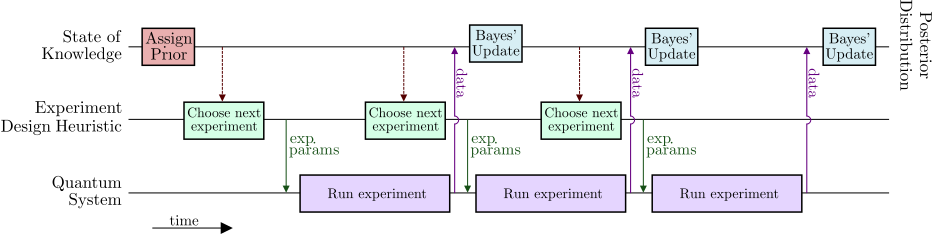
\includegraphics[width=\textwidth]{\figurefolder/online-timing-diagram}
    \caption{Timing diagram for three rounds of online learning. The role of the
    experiment design heuristic is to pick the next experiment, possibly based
    on the current state of knowledge (i.e. probability distribution over parameters
    of interest). This choice might be computationally expensive, and is 
    therefore run concurrently with quantum experiments.}
    \label{fig:online-timing-diagram}
\end{figure*}

%=============================================================================
\section{Conclusions}
\label{sec:conclusions}
%=============================================================================

Nulla commodo felis a est tincidunt porttitor. Praesent venenatis tellus eget ipsum tempus, sit amet tempus dui venenatis. Sed vel massa fermentum, cursus tellus ultricies, lacinia turpis. Donec rhoncus finibus semper. Pellentesque leo nunc, vehicula id tempor sit amet, tempus non nisi. Aliquam non faucibus nisi, quis dapibus odio. Duis ullamcorper nunc ultricies suscipit aliquam. Phasellus quis molestie eros, nec convallis justo. Integer massa diam, interdum quis diam ut, elementum luctus quam. Nullam interdum orci nec ultricies scelerisque. Praesent eget commodo tortor. In et risus vitae felis mollis hendrerit ut ac lacus. Maecenas congue sollicitudin erat, a eleifend nulla euismod ullamcorper. Nullam accumsan sodales metus. Vestibulum ante ipsum primis in faucibus orci luctus et ultrices posuere cubilia Curae; Pellentesque feugiat quam at justo tincidunt euismod. 

%=============================================================================
% END MATTER
%=============================================================================

\acknowledgments{
    
}

\nocite{apsrev41Control}
\bibliographystyle{apsrev4-1}
\bibliography{nv-adaptive}

%=============================================================================
% APPENDICES
%=============================================================================

\appendix
\onecolumngrid

%=============================================================================
\section{Effective Strong Measurements}
\label{apx:effective-strong-measurements}
%=============================================================================

Given a pre-measurement state $\rho$, information is accessed through the
Born's probability $p=\Tr(\ketbra{0}\rho)$.
In the hypothetical case of strong measurement, we would be able to draw from 
the Bernoulli distribution $\bernoullidist(p)$, or more generally, with 
$N$ repeated preparations and strong measurements, from 
the binomial distribution $\binomialdist(N,p)$.

Room temperature NV measurement does not allow strong measurements. 
Instead, our access to the quantity $p$ is obstructed by three Poisson rates,
such that conditional on some values $0<\beta<\alpha$, we can 
draw from the random variables
\begin{align}
    X|\alpha &\sim \poissondist(\alpha) \nonumber \\
    Y|\beta &\sim \poissondist(\beta) \nonumber \\
    Z|\alpha,\beta,p &\sim \poissondist(p\alpha + (1-p)\beta).
\end{align}
The information content about $p$ of such a measurement is not as obvious, 
and depends both on the magnitude of $\alpha$, as well as the contrast between 
$\alpha$ and $\beta$.

In this appendix, we introduce a measure we call the \textit{number of effective strong measurements} 
given some values of $\alpha$ and $\beta$.
This will allow us to make apples-to-apples comparisons between the obstructed
Poisson coin measurement and the binomial strong measurement which was mentioned initially.
It is important to stress that such comparisons are valid in the context of 
information gain and statistical inference alone; physically, nothing 
has changed, and the measurements are not strong.

Our strategy is conceptually simple. Given some estimate of $p$ 
made using variates of $X,Y,Z$, we calculate the number $N$ of strong measurements 
that would hypothetically result in the same uncertainty about $p$.
The word `uncertainty' is not precisely defined, and different interpretations 
will lead to different values of $N$.
At first, we consider the simplest case where the uncertainty is given by the variance 
of the respective maximum likelihood estimators, averaged uniformly over $p\in[0,1]$.
For the binomial case, this is easily computed as $\Var[\hat{p}]=p(1-p)/N$, equaling $1/6N$ when 
averaged over $p$.
For the referenced Poisson case, the Cramer-Rao bound provides a tight estimate 
in most regimes of $\alpha$ and $\beta$, with a formula given by~\citep{hincks_statistical_2017}.
\begin{equation}
    \Var[\hat{p}]\approx\frac{p(p-1)\alpha+(p-1)(p-2)\beta}{(\alpha-\beta)^2}
\end{equation}
which has an average value of $\frac{5(\alpha+\beta)}{6(\alpha-\beta)^2}$.
Equating these two variance formulas and solving for $N$ gives 
\begin{equation}
    N=\frac{(\alpha-\beta)^2}{5(\alpha+\beta)}
\end{equation}
which we define as the \textit{MLE number of effective strong measurements}.

TODO: generalize this to a Bayesian setting when we can incorporate prior
knowledge of $\alpha$ and $\beta$.
Then we should see an approximation to the above formula for $N$ in the case
of weak prior knowledge of $\alpha$ and $\beta$, and we should see an increase 
in $N$ if we have more precise prior knowledge.
The amount of increase is what I'm most interested in.

\end{document}
